\documentclass{article}
\usepackage{graphicx}

\title{Exploratory Data Analysis}
\author{Your Name}
\date{\today}

\begin{document}

\author{Joe Bloggs}

\maketitle{}

\section{Introduction}
This document presents an exploratory data analysis.

\section{Results}
Here is a sample figure:

\begin{figure}[h]
  \centering{
    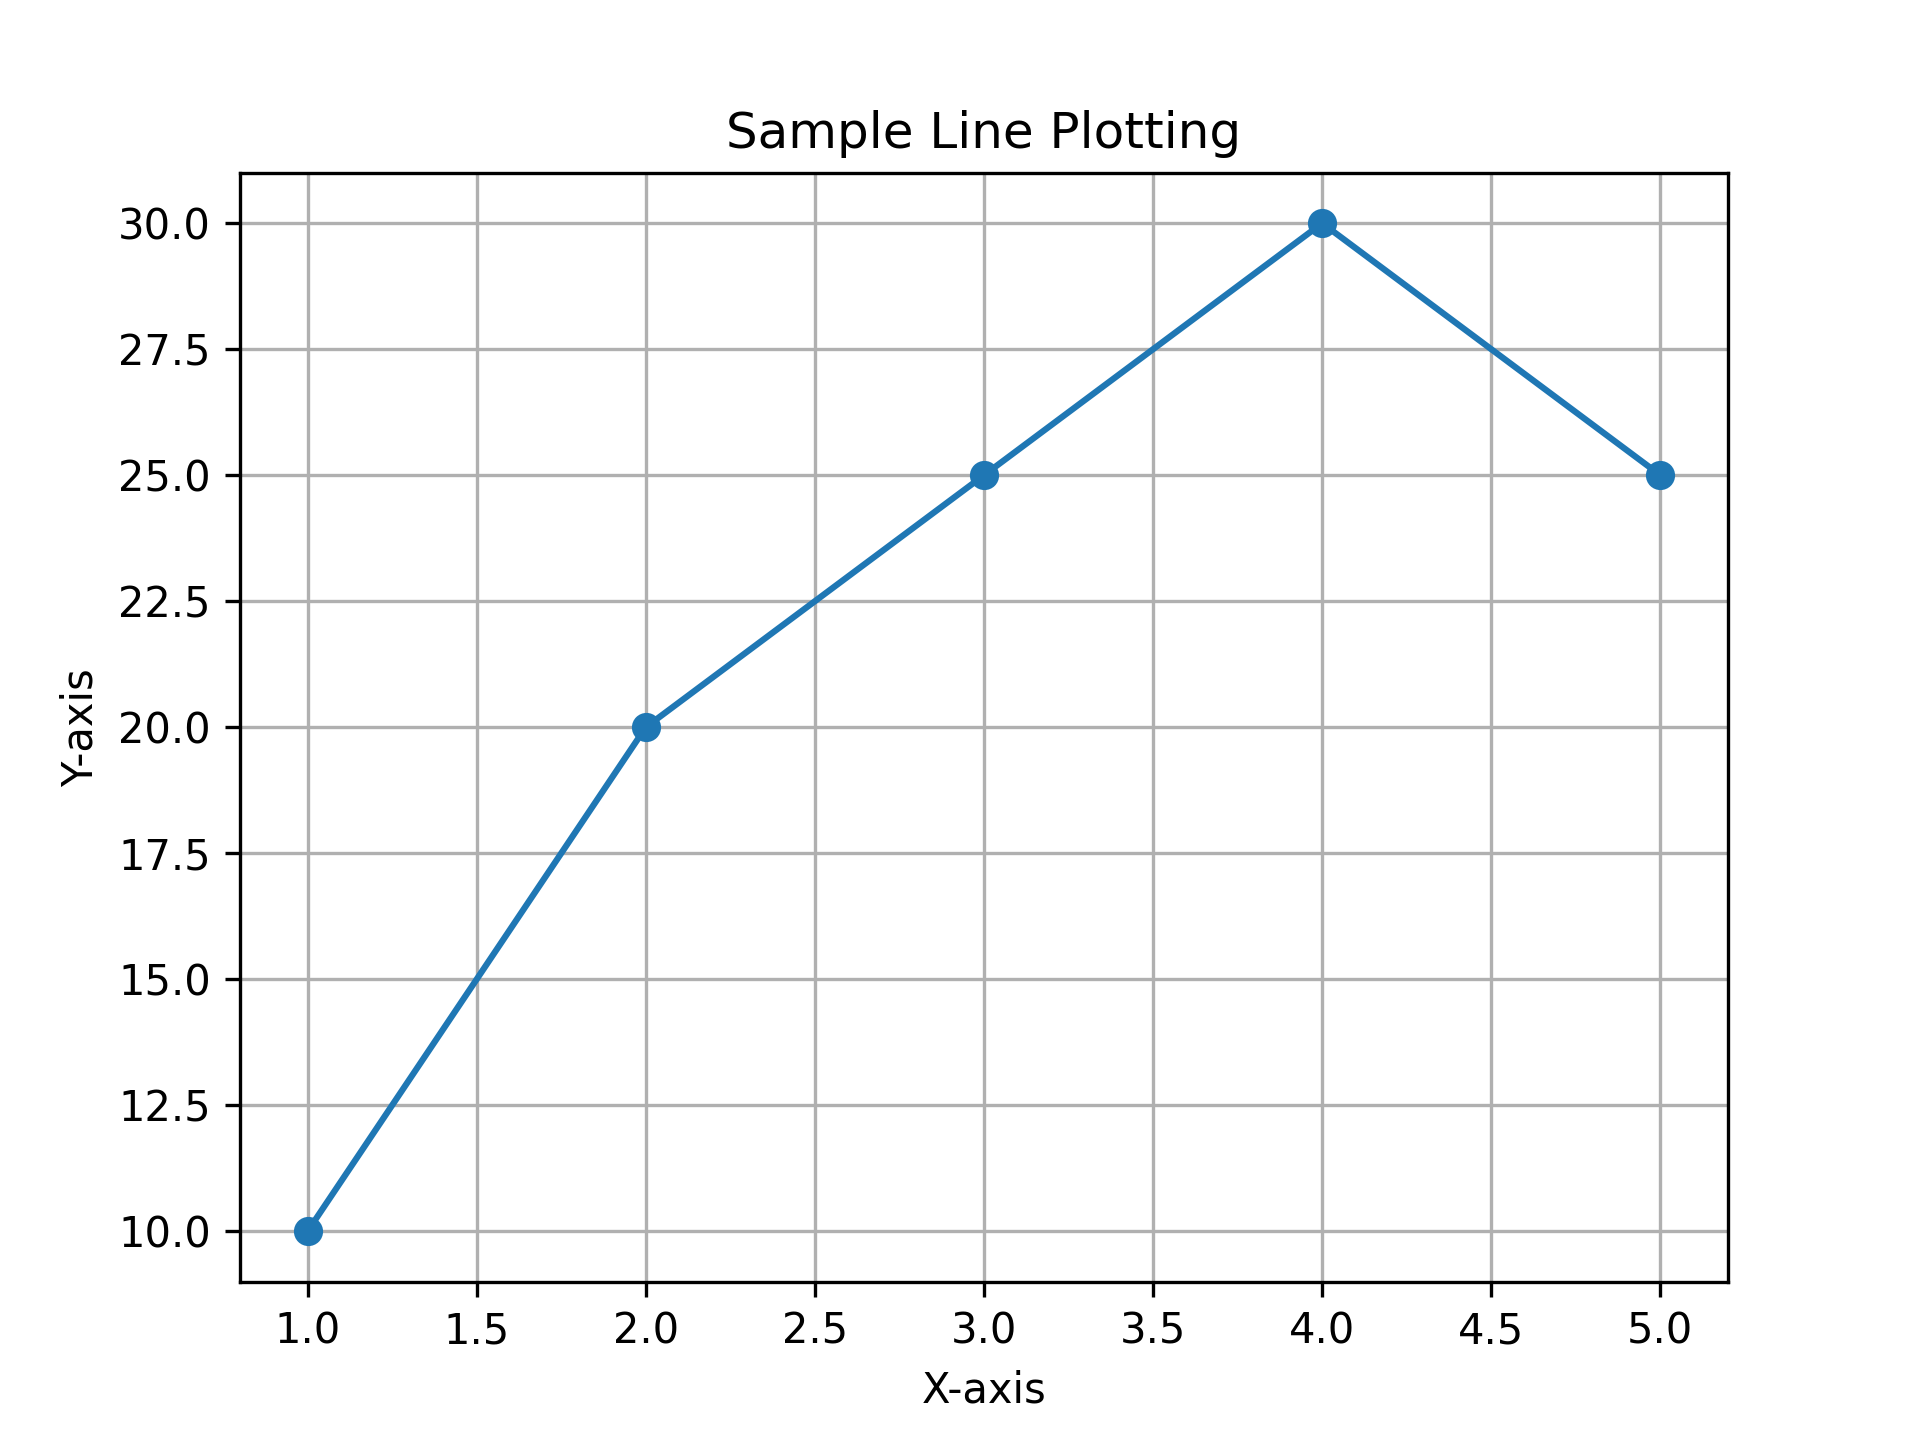
\includegraphics[width=0.5\textwidth]{figures/dummy_plot.png}
    \caption{Sample Plot}
    \label{fig:sample_plot}
  }
\end{figure}

% Example citations
As shown in \cite{smith2020example}, referencing is important.
Books like \cite{doe2019sample} and conference papers such as \cite{johnson2018conference} are also useful.
Miscellaneous sources can be cited as in \cite{random2021misc}.

% Bibliography
\bibliographystyle{plain}
\bibliography{dummy}

\end{document}